\documentclass{beamer}
%\usetheme[
%          titlepagelogo=bold50-illinois,% Logo for the first page
%          pageofpages=of,% String used between the current page and the total page count
%          titleline=true,% Show a line below the frame title
%          ]{TorinoTh}

\usetheme{Luebeck}

\usepackage{beamerthemesplit}
\usepackage{graphics}
\usepackage{graphicx}
\usepackage{hyperref}
\usepackage{comment}
\usepackage{ulem}
\usepackage{color} 
\usepackage{xspace}

\newcommand{\bllt}{\item \small}

\newcommand{\doneTask}[1]{\item \small \sout{#1}} 

\newcommand{\MyName}{Vivek~Kale} 

\newcommand{\fixme}[1]{\textcolor{blue}{[FIXME: #1]}}
\newcommand{\revision}[1]{\textcolor{blue}{[FIXME comment : #1]}}

\title{Notes}
\author{\MyName}
\date{\today}

\title[All Notes]{Prelim Outline Notes }
\author[Vivek Kale]{%
  Vivek~Kale\inst{1}}

\institute[University of Illinois at Urbana-Champaign]{
  \inst{1}%
  Department of Computer Science\\
  University of Illinois at Urbana-Champaign
}
\date[DLT 2012]{\today}
\subject{Computational Sciences}

\begin{document}
\AtBeginSection[] 
{
\begin{frame}
\frametitle{Outline}
\tableofcontents[part=1, pausesections]
\end{frame}
}

\titlepage
\section{Prelim Outline Notes}
\begin{frame}
\frametitle{Intro}
\begin{enumerate} 
\item \tiny 
\item \tiny 
\end{enumerate} 
\end{frame}


\begin{frame}
\frametitle{ Problem} 
\begin{itemize}
\item \tiny Performance Irregularities inhibit performance for current generation and next-generation hpc clusters. \\ 
\item \tiny One particular example of performance irregularity is noise. Others could be load imbalances without a pattern. \\ 
\item \tiny We can see this through simulation, through Hoefler et. al. where 1 million MPI processes were simulated, and amplification was shown to occur. \\ 
\item \tiny We see this through theory, through Tsasfir et. al where noise amplification is shown through probabilistic analysis ,  using real machine parameters to show effects of amplification at large scales. \\
\item \tiny We see this through experimentation, as shown in Petrini et. al.  where the effect of noise amplification is shown on 8192 processors.  \\
\end{itemize} 
\end{frame}

\begin{frame}
\frametitle{Details on Problem: Sharing an SMP}
\begin{columns} % contents are top vertically aligned                                                                                                                                  
%\begin{column} % each column can also be its own environment                                                                                                                                                                                                                                  
\column{0.5\textwidth}
\begin{itemize}
\tiny \item \tiny Having many cores available makes everyone think that  
they can use them to solve other problems (“no one would use all of them all of the time”).  \\  
\item \tiny However, compute-bound scientific calculations are often written as if all compute  
resources are owned by the application. \\ 
\item \tiny Such static scheduling leads to performance loss. \\ 
\item \tiny Pure dynamic scheduling adds overhead, but is better. \\ 
\item \tiny Careful mixed strategies are even better. \\ 
\item \tiny Recent results give 10-16\% performance improvements on large, scalable systems. \\  
\end{itemize}
\column{0.5\textwidth}
% alternative top-align that's better for graphics                                                                                                                                                                                                                                                     
%\framebox{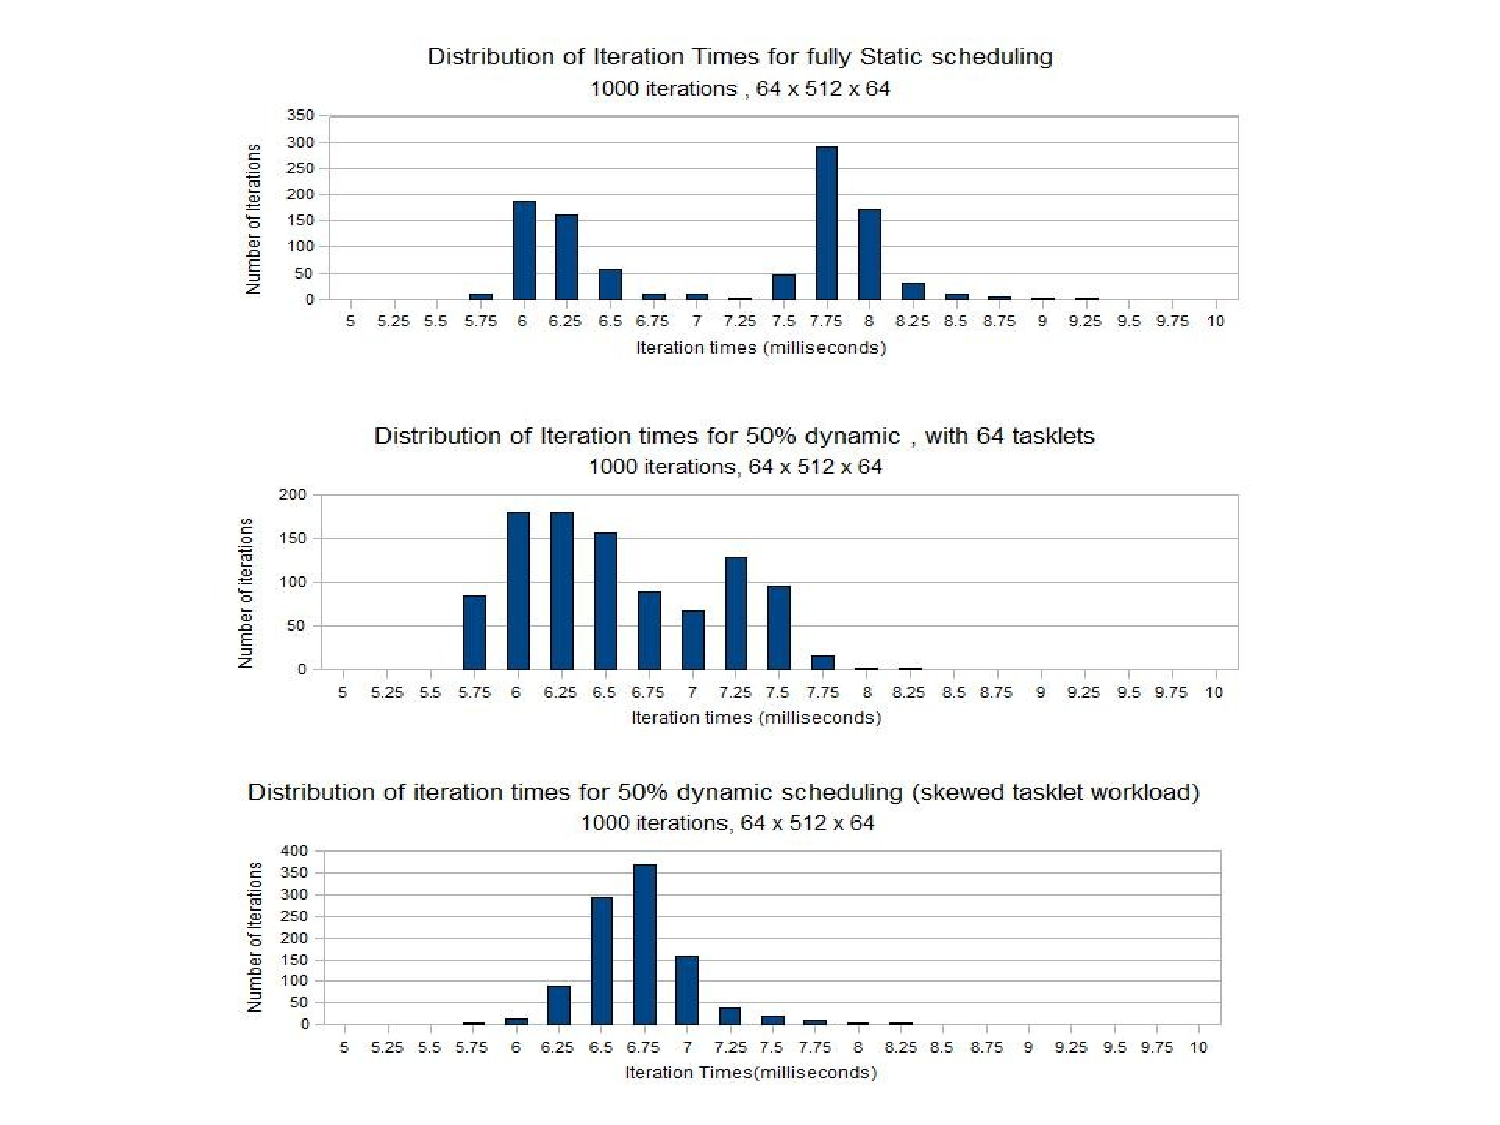
\includegraphics[scale=0.22]{images/uSched-signature-graph}}                                                                                                                                                                                                                                   
\framebox{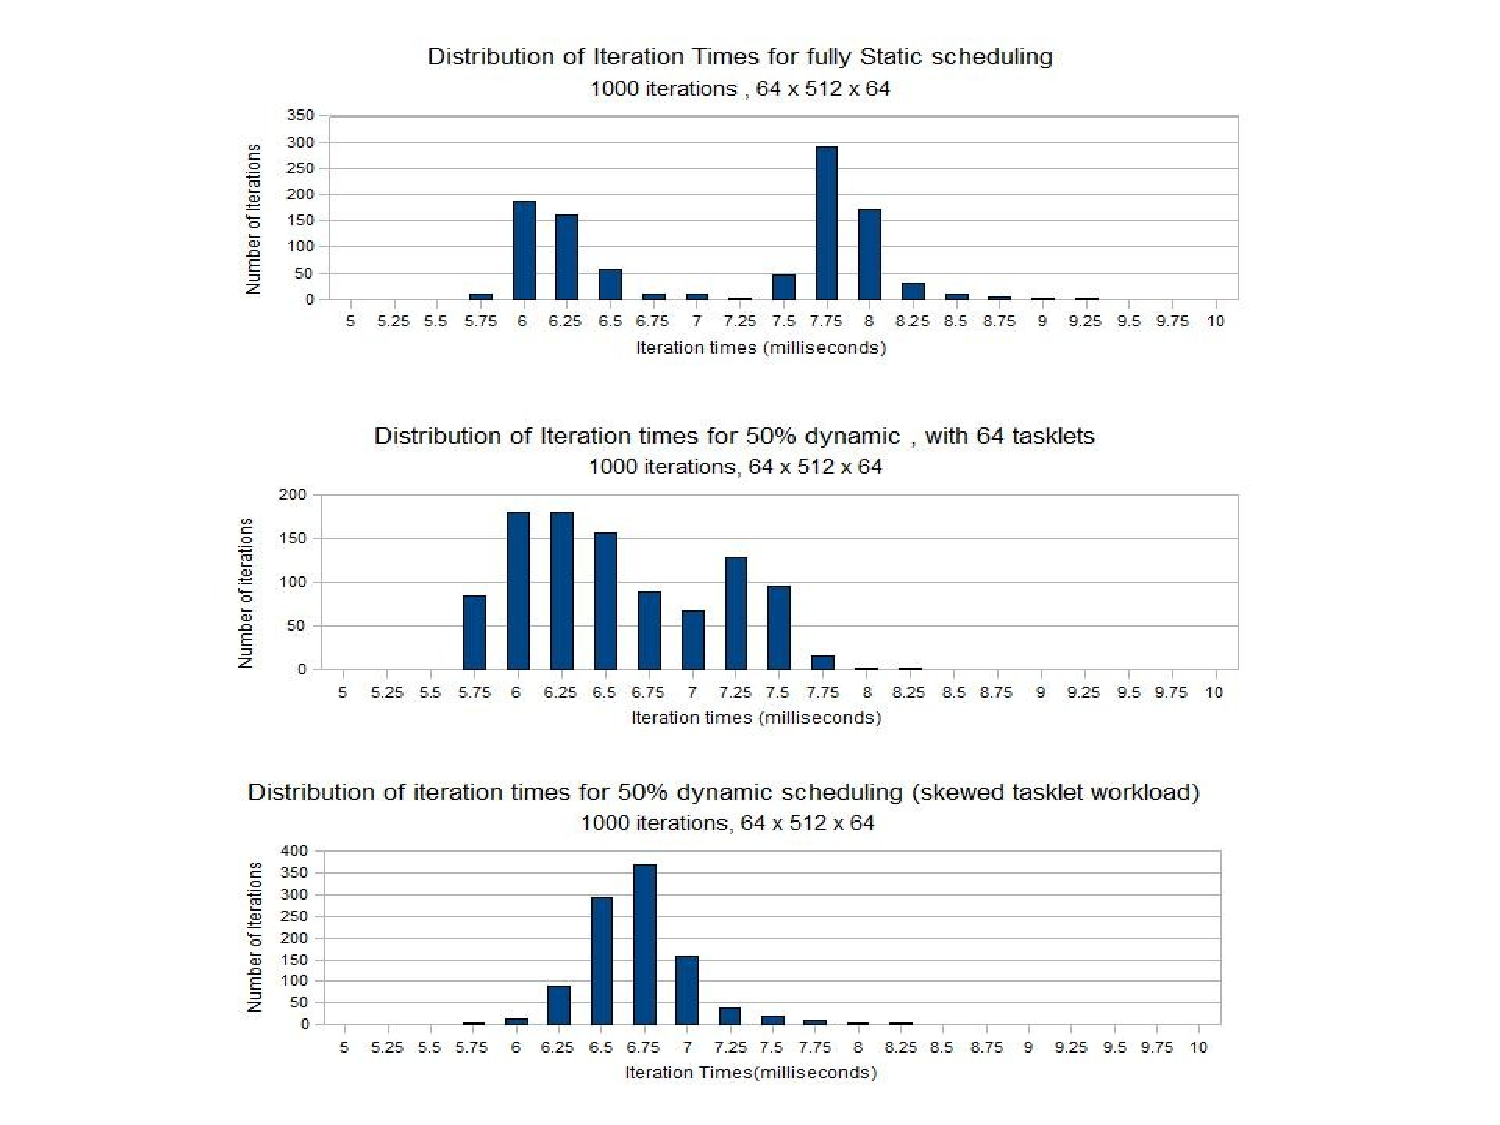
\includegraphics[width=\textwidth]{images/uSched-signature-graph}}
\end{columns}
\end{frame}

\begin{frame}
\frametitle{Details on Problem: The Performance Irregularity Amplification Problem}
\begin{itemize}
\item \small Each node has unpredictable, \textit{excess work},
which we call ``noise''.  \\
\item \small The resulting load imbalance is  \textit{uncoordinated},
  \textit{localized}, and \textit{transient} (U.L.T.).  \\
\item \small This noise is negligible for a program running on a single node. \\
\begin{itemize}
\item \small For example, 0.1\% overhead.
\end{itemize}
\item However, with dependences in MPI applications, especially via collective communication,
if one core of a node experiences U.L.T. event in a timestep, the global timestep is slowed down.
\begin{itemize}
\item \small All other nodes wait for the affected node to finish.
\end{itemize}
\item \small So, as we increase the number of nodes, it becomes increasingly likely that
\textit{some} core will experience a U.L.T. event, in each timestep.
\item \small The 0.1\% overhead becomes amplified to a much larger fraction.
\begin{itemize}
\item \small depending on the amplitude of the U.L.T. event,
and the duration of the application timestep.
\end{itemize}
\end{itemize}
\end{frame}
-
\begin{frame}
\frametitle{Why Other Soln's don't work(listed in order of innovation date) } 
\begin{enumerate} 
\item \small Co-scheduling can't always help because it is hard to schedule everything together, as some nodes will have timers. Also, can't coschedule hardware variations. 
\item \small Low-noise OS can't help because there may be noise coming from the runtime system.  
\item \small Extra core (as on BG/Q) can't always help because there are other noise events that may be coming from 
\item \small Since performance irregularities are essentially a load imbalnce, basic dynamic scheduling is one solution to help mitigate this problem.  
\begin{itemize}
\item \tiny Cilk Work-stealing 
\item \tiny OpenMP dynamic scheduling
\end{itemize}
\end{enumerate} 
\end{frame} 


\begin{frame}
\frametitle{How do we solve this problem?} 
\begin{enumerate} 
\item \small Our basic solution: use lightweight scheduling to dampen occasional noise within one node. 
\item \small Our basic solution: use lightweight scheduling to dampen occasional noise within one node. 
\end{enumerate} 
\end{frame} 


\begin{frame}
\frametitle{Our Core $\mu$-scheduling Solution: Motivation}
\begin{itemize}
\item Exploit multiple cores on a node: distribute the excess work on
the core affected by noise to the other cores dynamically.
\begin{itemize}
\item {\small Create \textit{tasklets} and schedule them dynamically.}
\end{itemize}
\item Optimizations:
\begin{itemize}
\item {\small Making all work dynamic has high overhead
 (enqueue/dequeue, lock). Thus, we make last fraction
of work dynamic (the rest is static).}
\item {\small Dynamic scheduling interferes with locality across timesteps.
Thus, we keep track of the core that executed it last iteration, and try to keep work on that core. }
\end{itemize}
\end{itemize}
\end{frame}

\begin{frame}
\frametitle{MPI Domain Decomposition for 3D Stencil}
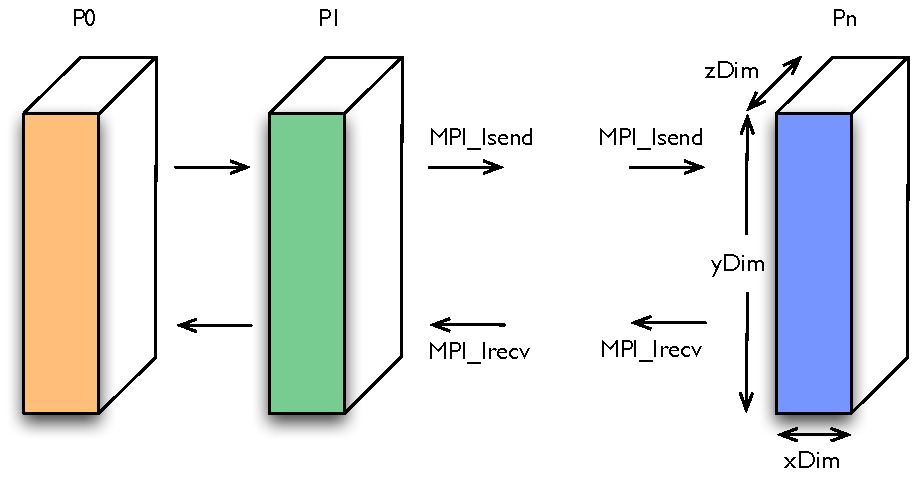
\includegraphics[width=\textwidth]{images/mpi_decomp}
\end{frame}

\begin{frame}
\frametitle{Using Our Core $\mu$-scheduling Solution}
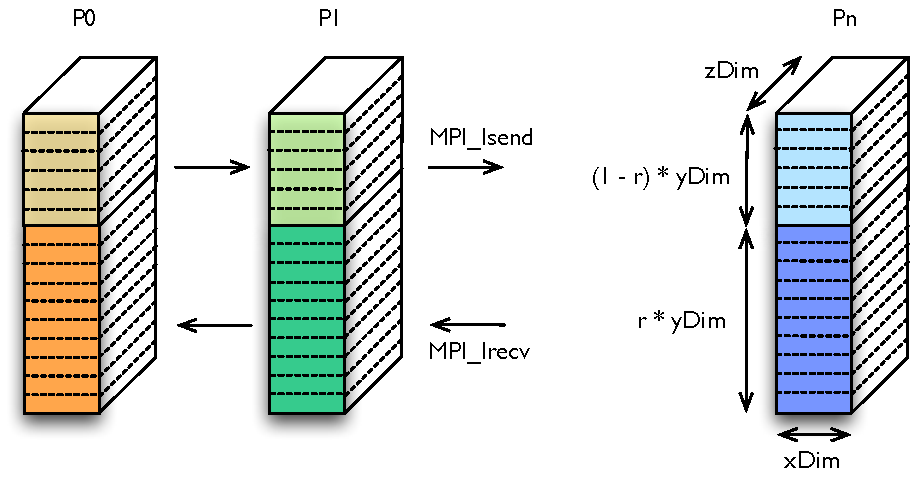
\includegraphics[width=\textwidth]{images/hybrid_decomp}
\end{frame}


\begin{frame}
\frametitle{Defining Problem Space} 
\begin{enumerate} 
\item  \small The problem space is for applications such as LU factorization, PDE's which can have fast computations. 
\item \small Something like Quantum Monte Carlo can do with heavyweight mechanisms. 
\item \small 
\end{enumerate} 
\end{frame}


\begin{comment}
\begin{frame}
\frametitle{What we are trying (and not trying) to do } 
\begin{enumerate} 
\item  
\item 
\item 
\end{enumerate} 
\end{frame} 
\end{comment}



\begin{frame} 
\frametitle{Justification of our solution}
\begin{itemize} 
\item \small Within node is sufficient because once you go off-node,
  the cost of coherence cache misses is very high, making it very hard
  to make a lightweight mechanism work. 
\item \small Importance of lightweight (and why pure virtualization
  approaches are not always adequate): pure virtualization is not
  adequate due to cost of communication latency being high. 
\item \small Pure virtualization is not adequate due to cost of
  communication latency being high. 
\item \small Measurement-based load balancing not sufficient due to
  not being able to predict noise patterns a priori (as noise is a
  transiently varying quantity). 
\end{itemize}
\end{frame}


\begin{frame}
\frametitle{Perf. Model for noise}  
\begin{itemize} 
\item \small (obtain from docs)
\item 
\item 
\end{itemize}
\end{frame}


\begin{frame}
\frametitle{Perf. Model for Dynamic Scheduling}  
\begin{itemize} 
\item \small (obtain from docs)
\item 
\item 
\end{itemize}
\end{frame} 

\begin{frame}
\frametitle{Perf. Model for MPI Slack}  
\begin{itemize} 
\item \small (obtain from docs)
\item \small 
\item \small 
\end{itemize}
\end{frame} 


\begin{frame}
\frametitle {How can scheduling decisions be made? }
\begin{enumerate}
\item \small \textbf{Compile time:} 
\begin{itemize} 
\item \tiny Tune static fraction. 
\item \tiny Tune tasklet size
\end{itemize}
\item \small \textbf{Runtime:}
\begin{itemize} 

\item \tiny Implementation of new scheduler which decides how tasklets are distributed in the queue. 
\end{itemize}
\item \small \textbf{Across Runs:}
\begin{itemize} 
\item \tiny Each core/thread has preference for tasklets that run on it from before.  
\item \tiny We can use patterns in persistent noise to make decisions
  about weighting work from one core to the other. 
\item \tiny We can use knowledge of slack to further avoid scheduling,
  because we know we won't amplify when there it is known to have
  adequate slack. 
\end{itemize}
\end{enumerate}
\end{frame}

\begin{frame}
\frametitle{Algorithm for lightweight Scheduling} 
\begin{enumerate} 
\item \small Our basic solution: use lightweight scheduling to dampen
  occasional noise within one node. 
\end{enumerate} 
\end{frame} 

\begin{frame} 
\frametitle{Algorithm for Slack-conscious lightweight Scheduling} 
\begin{enumerate} 
\item \small Our basic solution: use lightweight scheduling to dampen
  occasional noise within one node. 
\end{enumerate} 
\end{frame} 

\begin{frame}
\frametitle{Implementation for lightweight Scheduling} 
\begin{enumerate} 
\item \small 
\item \small 
\item \small 
\end{enumerate} 
\end{frame} 

\begin{frame}
\frametitle{Implementation for Slack-conscious Lightweight Scheduling} 
\begin{enumerate} 
\item \small 
\item \small 
\item \small 
\end{enumerate} 
\end{frame} 

\begin{frame}
\frametitle{Problem/Issue --> Solution}
\begin{itemize}
\item \small Overhead of scheduling when task size is computationally
  small --> \textit{extremely lightweight scheduling, including compile-time}. 
\item \small  Importance of locality --> \textit{take locality into account in
  decisions, while remaining lightweight}.
\item \small Predicting performance imbalance is hard --> observe
  correlation with communication delays --> use slack. Etc.  
\end{itemize} 
\end{frame}


\begin{frame}
\frametitle{Sched} 
\begin{table}[h!]
  \begin{center}
    \small
    \begin{tabular}{ | c || c | c | c | c | c | c | c |}
      \hline
      & \underline{T1} & \underline{T2} & \underline{T3} & \underline{T4} & \underline{T5} & \underline{T6} & \underline{T7} \\ 
      \hline
      \tiny \textbf{I1(<weight>)}  &  \tiny - &\tiny -  & \tiny - & \tiny -  & \tiny -  & \tiny - & \tiny - \\ 
     \hline
      \tiny \textbf{I2(<weight>)}  &  \tiny - &\tiny -  & \tiny - & \tiny -  & \tiny -  & \tiny - & \tiny - \\ 
      \hline
      \tiny \textbf{I3(<weight>)}  &  \tiny - &\tiny -  & \tiny - & \tiny -  & \tiny -  & \tiny - & \tiny - \\ 
      \hline
    \end{tabular}
  \end{center}
  \caption{<Table Caption goes here>}
\end{table}
\end{frame} 


\begin{frame} 
\frametitle{Thesis Committee} 
\begin{enumerate}
\item \small Maria Garzaran 
\item \small Prof. Wen-mei Hwu OR Prof. David Padua
\item \small Prof. William Gropp
\item \small  Bronis de Supinski
\end{enumerate}
\end{frame} 

\begin{comment}
\begin{frame}
\frametitle{}
\begin{enumerate}
\item \small \textbf{Item A}
\begin{itemize} 
\item \tiny 
\item \tiny
\end{itemize} 
\item \small \textbf{Item B}
\begin{itemize} 
\item \tiny re-imbursements
\item \tiny 
\item \tiny 
\end{itemize} 
\item \small \textbf{Item C} 
\begin{itemize} 
\item \tiny 
\item \tiny 
\item \tiny 
\end{itemize} 
\end{enumerate}
\end{frame}   
\end{comment}

\end{document} 
